%\documentclass[a4paper,12pt]{report}
\documentclass[twoside,12pt]{uafthesis}


%allows for hyperlink
\usepackage{hyperref}
%re-define how \autoref (found in hyperref package) prints a chapter reference
%Default is "chapter", but I want "Chapter" instead
\renewcommand*{\chapterautorefname}{Chapter}
\renewcommand*{\subsubsectionautorefname}{subsection}
%\usepackage{url}

%allows for degree symbol, among other things presumably
\usepackage{textcomp}

%allows for the construction of a nomenclature section
\usepackage[intoc]{nomencl}
%\usepackage{nomencl}
\makenomenclature
\setlength{\nomitemsep}{0.0em}
\renewcommand{\nomname}{List of Symbols}
\newcommand{\nomunit}[1]{%
	\renewcommand{\nomentryend}{\hspace*{\fill}#1}}
\renewcommand{\nompostamble}{%
	\cleardoublepage}
\makeatletter
\def\thenomenclature{%
	\@chapteronefalse
	\if@arabic\relax\else\renewcommand{\thepage}{\roman{page}}\fi
	\chapter*{\nomname
		\@mkboth{\uppercase{\nomname}}%
				{\uppercase{\nomname}}}
	%\@chapteronetrue
	\if@intoc\addcontentsline{toc}{section}{\nomname}\fi%
	\nompreamble
	\list{}{%
		\labelwidth\nom@tempdim
		\leftmargin\labelwidth
		\advance\leftmargin\labelsep
		\itemsep\nomitemsep
		\let\makelabel\nomlabel}
	%\nompostamble
	%\list{}{%
	%	\newpage\renewcommand{\thepage}{\roman{page}}}
}
\makeatother

%for grouping withing nomenclature section
\usepackage{etoolbox}
\renewcommand\nomgroup[1]{%
	\item[\bfseries
		\ifstrequal{#1}{V}{Variables}{%
		\ifstrequal{#1}{S}{Subscripts}{%
		\ifstrequal{#1}{B}{Acronyms}{}}}%
	]}



%draws bounding boxes around the major page elements. For troubleshooting
%\usepackage[showframe]{geometry}


%allows multiple rows in a single column withing a table
\usepackage{multirow}

%allow row shading in table environments
\usepackage[table]{xcolor}

\usepackage{amsmath, amssymb, amsfonts} % Thanks, AMS!
%\usepackage{fixltx2e} % Allows \(\) in captions, amongst other things.
%\usepackage{ppl} % The Paladino font (tough to find?)
%\usepackage{pxfonts} % Paladino-like fonts
\usepackage{graphicx, float} % Graphics stuff
\usepackage[space]{grffile}
\usepackage{verbatim} % Mostly for the comment environment.
%\usepackage{chapterbib} % This is an option for those bundling papers.
%\usepackage[square]{natbib}
%\usepackage{tocbibind} % This fixes the "bibliography in ToC" problem.
                        % Use with chapterbib.
\usepackage{booktabs}                       
\usepackage{cancel}
%\usepackage{caption}
\usepackage{cleveref}
\usepackage{colortbl}
\usepackage{csquotes}
\usepackage{helvet}
\usepackage{mathpazo}
\usepackage{listings}
\usepackage{pgfplots}

%\usepackage{translator}
%\usepackage{beamer}

%For using units in equation mode 
\usepackage{siunitx}
\DeclareSIUnit\rpm{rpm}
\DeclareSIUnit\gpm{gpm}
\DeclareSIUnit\voltamp{VA}
\DeclareSIUnit\voltampreactive{VAR}
\DeclareSIUnit\degreeFahrenheit{\degree{}F}

%Allows for drawing circuit diagrams
%\usepackage[siunitx]{circuitikz}
\usepackage[american]{circuitikz}

%allows writing of chemical formulea
\usepackage{chemformula}


%Not sure exactly why this line is needed but I got a warning that said: running in backwards compatibility mode (unsuitable tick labels; missing features). Consider writing \pgfplotsset{compat=1.16} into your preamble.
\pgfplotsset{compat=1.16}

%certain default hyphenations aren't what I want
\hyphenation{geo-ther-m-al}

%NO WIDOWED OR ORPHANED LINES
\widowpenalty10000
\clubpenalty10000

%Various title/signature page info
\author{Nathan Green}
\title{Modeling and Analysis of Geothermal Organic Rankine Cycle Turbines coupled with Asynchronous Generation as a Primary Power Source in Islanded Microgrids}

\degreeyear{2019}
\degreemonth{May}
\degree{Master of Science}
%\degreesubject{Electrical Engineering}
\department{Electrical \& Computer Engineering}
\numberofmembers{3} % Make sure this is right! The grad school hates empty
                    % signature lines.
\committeechair{Richard Wies}
\committeememberfirst{Daisy Huang}
\committeemembersecond{Mari Shirazi}
\departmentchair{Charlie Mayer}
\collegedean{William Schnabel}
\graddean{Michael Castellini}

\committeewidth{4in}
\approvedwidth{4in}
\comitteespace{\hfill}
\approvedspace{\hfill}

\prevdegrees{B.S.}
\college{College of Engineering \& Mines}


\begin{document}
\pagenumbering{roman}
%\makesig
\maketitle
\begin{abstract}

Diesel electric generation is heavily used in remote permanently islanded microgrids, even in areas where alternative resources are readily available. The cost of diesel fuel for these generators is high in part because of the difficulty in transportation. Additionally, as the cost of fuel increases, so too does the cost of transportation, hitting these remote communities harder. This thesis will show that local resources such as geothermal hot springs can provide primary for these remote microgrids, even at relatively low temperatures below the boiling point of water. The geothermal heat will be processed with organic Rankine cycle in combination with a self excited induction generator. A steady-state energy balance model will be devoloped using MATLAB Simulink. The model will be used to simulate greenfield and brownfield geothermal microgrids at Pilgrim Hot Springs, Alaska and Bergssta$\eth$ir, Iceland respectively to demonstrate viability of this microgrid design. 

%A stability analysis will be conducted using the long and short term simulation models which evaluate system voltage and frequency under different conversion topologies. A cost analysis will also be conducted to compare the economic viability of operating the different systems in remote communities. It is expected the system with greatest stability will not be the most cost-effective, but that there is a system which provides stable power within reasonable tolerances at optimal cost.

\end{abstract}

\begin{acknowledgements}
	I would like to thank \dots
	
	 My friends \& family for helping cultivate the person who I have become. 
	 
	 All the members of my committee, both past and present, for guiding me. 
	 
	 Everyone at ACEP for supporting me. 
	 
	 And Sarah for inspiring me.
\end{acknowledgements}


%Table of Contents and such
\tableofcontents
\listoffigures
\listoftables
%\listofothermaterials
%\listofappendices
%\cleardoublepage% or \clearpage
%\pagenumbering{roman}
%\setcounter{page}{13}
%\addcontentsline{toc}{section}{\nomname}

%\markboth{\nomname}{\nomname}% maybe with \MakeUppercase
\printnomenclature[0.75in]

%\cleardoublepage


%\pagenumbering{arabic}
%Each chapter is included
\chapter{Introduction}
\label{ch:intro}

\section{Problem Statement}
The state of Alaska currently has dozens of communities which are electrically isolated from the rest of the state. They effectively act as remote permanently islanded microgrids. These communities typically use diesel generators to provide most of their electrical power. Power sources such as coal or natural gas are less expensive in larger grids, but these microgrids are too small to take advantage of such economies of scale. This makes it expensive to operate relative to the size of the communities. Furthermore, the remoteness of these communities significantly increases the cost to import fuel.

The goal of this thesis is to determine an affordable method to incorporate renewable energy into microgrids without compromising stability and reliability. One method of reducing operating costs is to offset diesel fuel through the use of locally available renewable energy resources.\footnote{Sometimes called renewables, these sources of energy either will not be depleted or can be replenished in a reasonably short period of time. They include wind, solar, geothermal heat, biomass, and water flow.} Unfortunately powering a microgrid with a significant portion of intermittent renewable resources can negatively impact grid stability unless appropriate infrastructure is included. 

This thesis will seek to accomplish its goal by simulating the operation of a permanently islanded microgrid containing geothermal organic Rankine Cycle (ORC) power generation for two types of site applications. In both cases the geothermal power will be converted from AC to DC then back to AC in to be distributed to the loads.
\begin{itemize}
\item One greenfield site will be examined with no existing permanent electrical infrastructure.
\item One brownfield site will be examined where there is an existing grid connection but experiences regular outages.
\end{itemize}
\nomenclature[B]{ORC}{Organic Rankine cycle}

The greenfield area selected for this study, Pilgrim Hot Springs, lies about 60 miles north of Nome in western Alaska. Since the 1970s there has been interest in developing the hot springs in order to generate electricity.  Several exploratory wells have been drilled and indicate potential for low temperature geothermal electrical generation \cite{Holdmann2013}. \autoref{fig:pilgrimFLIR} shows a geothermal runoff stream and how much warmer the water is compared to the banks. The area is currently undeveloped,\footnote{There are historic ruins of an old church and orphanage from the early 1900s, but those buildings are uninhabitable.} therefore, this remote microgrid will be designed from scratch. The land owners, Unataaq LLC, have expressed interest in developing the resource as a tourist attraction, for agriculture, as well as for electrical production. They are currently working with the Alaska Center for Energy and Power (ACEP), a research group at the University of Alaska Fairbanks, to fulfill these goals. 
\begin{figure}[h]
	\centering
	
	\includegraphics[width=\textwidth]{figures/PilgrimFLIR.png} 

	\caption{A FLIR image of a Pilgrim hot springs geothermal runoff stream overlayed onto a photo.}
	\label{fig:pilgrimFLIR}


\end{figure}
\nomenclature[B]{ACEP}{Alaska Center for Energy and Power}

The greenfield system would be similar to the organic Rankine cycle generator used in Chena Hot Springs. Though near Fairbanks, Alaska, these hot springs are not connected to the larger grid, and primarily use diesel generators to produce electric power. In an effort to reduce fuel usage, the owner worked with United Technologies and Carrier Refrigeration to install two 200 kW ORC generators to supplement the diesel generation. At the time of construction, the system found at Chena Hot Springs made use of the lowest temperature geothermal resource for operating ORCs \cite{Holdmann2007}. In addition to the ORCs, Chena uses the geothermal hot water to heat cabins and greenhouses, as well as for sitting pools. 

Iceland has extensive experience utilizing their geothermal resources, but so far only high temperature areas are used for electricity production, while low temperature sites are used for district heating. One such system, and the brownfield case study, heats the community of Bergsta$\eth$ir, Iceland, a rural area in the northern part of the island. \autoref{fig:bergstadir_effluent} shows the discharge pipe and steaming effluent of the system. The pumps used to circulate the water are electrically driven by two \SI{15}{\kilo\watt} motors, but the electrical grid in rural Iceland is less reliable than the heating loop needs to be. Currently the community uses diesel generators to power the pumps during the power outages, but they are interested in alternatives.
\begin{figure}[h]
	\centering

	\includegraphics[width=\textwidth]{figures/BergstadirEffluent.jpg} 

	\caption{District heating effluent at Bergssta$\eth$ir, Iceland. Credit: George Roe.}
	\label{fig:bergstadir_effluent}

\end{figure}

\autoref{fig:abridged_flow_diagram_label} shows a simplified flow diagram of the model using an ORC as the power source. The components include an ORC system as a source, a load, and an inverter to link the source output to the load. In the figure, the blue lines represent electrical connections, while green represents the flow of data and component parameters. The ORC block is composed of evaporating and condensing heat exchangers, an isentropic pump, an isentropic expander, and self-excited induction generator. 
\begin{figure}[ht]
	\centering
	\caption{A simplified diagram of power and data flows of the model. Blue lines represent electrical power connections and flows similar to a one-line diagram. Green boxes data flow from one part of the model to another.}
	\label{fig:abridged_flow_diagram}
	
	%\includegraphics[width=\textwidth]{figures/Abridged Pilgrim Model Flow diagram - AC bus.pdf} 
	\includegraphics[width=\textwidth]{figures/SimpleFlowDiagram.pdf}

\end{figure}

\section{Microgrid Description}
Microgrids are electrical systems composed of sources and loads within a well defined electrical boundary. Many microgrids are connected to a larger grid, but with the ability to become separated, or islanded, while still maintaining some or all of the loads. Others need to remain connected but still maintain a boundary. Some form of energy storage is often used for systems operating independently from the larger grid. This section will describe the key components and characteristics of a microgrid with emphasis on relevance to Alaska.

Approximately 70\% of the population of Alaska is connected to a single grid called the Railbelt \cite{railbelt}. The Railbelt stretches over 600 miles from Homer on the Kenai Peninsula to the greater Fairbanks area in the interior and includes most communities on the road system. The remaining communities and villages can be considered permanently islanded microgrids. Each has loads that need power, some power source, and some system of storing the energy or fuel.

A microgrid can operate using alternating current (AC), direct current (DC), or a hybridization of the two. The choice of whether to use AC\footnote{Unless otherwise noted, AC will refer to three phases separated by a phase angle of 120\textdegree{} rather than a single phase.} or DC depends on the demand of the loads, the available power sources and conversion devices, as well as the existing electrical infrastructure. The decision between AC and DC goes as far back as 1880s when George Westinghouse and Thomas Edison were competing to supply America with electrical power. Ultimately Westinghouse and AC came out on top in part due to its relative ease of transforming to high voltage and low current which transmits more efficiently. Furthermore, electric machinery that uses AC to generate rotating magnetic fields operates more efficiently than machines which use DC power and commutators. Like most of the world, Alaska uses AC networks and converts to DC as necessary at the device level.
\nomenclature[B]{AC}{Alternating current}
\nomenclature[B]{DC}{Direct current}

While AC is still the standard for most power distribution and transmission, DC applications are seeing increased attention. DC interties are already used to connect large areas of the national power grid to act as a buffer for frequency and voltage variations between each part of the system. DC microgrids also have the potential to improve stability with distributed, intermittent, and highly variable renewable generation, although much work is still needed. Integration of AC and DC infrastructure remains challenging for adaption into existing systems, though low-cost solid-state power electronic converters increase the viability of greenfield DC microgrids.
%More recently, however, computers and other electronic devices which use DC have become much more prolific, which has led to a renewed call for DC systems. 

\subsection{Sources}
Microgrid power is typically generated by distributed energy resources (DER). This can include renewable resources such as solar photovoltaics, wind turbine generators, hydrokinetics, biomass, and geothermal-based generators. Some non-renewable DERs include diesel generators and natural gas micro-turbines. 
%Most power sources generate AC power. Current is induced by rotating coils withing a magnetic field
\nomenclature[B]{DER}{Distributed energy resource}

Diesel generators use the combustion of diesel fuel to spin an alternator producing AC power. These generators are prolific in rural Alaska generally being used as the prime mover to regulate grid frequency and voltage. The communities  generally purchase the fuel in bulk once or twice each year because of their remote locations. The fuel is then stored in tank farms.
%These generators are composed of an engine, alternator, fuel system, excitation system, governor, cooling system, exhaust system, and turbocharger.
Due to the widespread use of diesel generators in Alaska, significant energy cost savings can be generated by reducing fuel consumption through efficiency improvements and use of renewable energy sources. 

This thesis is focused on using geothermal generators, in particular, as a prime renewable energy source to displace the fuel consumption of diesel generation. Geothermal generators are heat engines, and operate similarly to traditional coal and nuclear plants. Heat causes a working fluid to thermally expand and change phases thus spinning a turbine to produce AC power. The primary difference is that geothermal systems get heat from the Earth as opposed to combustion or nuclear reactions. Geothermal generators can be divided into high heat and low heat categories. High heat geothermal systems work with temperatures well above the boiling point of water which means water can be used as the working fluid. Low heat systems operate at temperatures near or below the boiling point of water therefore a refrigerant must be used as an alternative working fluid. 
%talk about chena hotspings as an example of existing geothermal in AK

%Wind turbine generators produce what is known as wild AC, where frequency and voltage are unregulated and can vary with wind speed. Modern wind turbines have built-in methods of ensuring the generated power is usable by the grid.
%\begin{verbatim} 
% address gearboxes  
% various wind turbine conversion topologies perhaps
% talk about wind resources of western alaska
%\end{verbatim}

%Solar photovoltaic (PV) panels generate DC power. Panels are made up of a string of cells of a semiconductor material. The most commonly used material is Silicon, but Gallium Arsenide (GaAr), Cadmium Telluride (CdTe), and Copper Indium Gallium Selenide (CIGS) can be used in certain applications as well. Regardless of the material, all PV panels operate by absorbing sunlight and exciting electrons to higher energy orbital. Some fraction of the excited electrons become free and capable of generating a current. PV systems in Alaska face certain challenges due to the long dark winters, however there are also several beneficial characteristics. Solar PV cell operate more efficiently in colder temperatures and reflection due to high albedo of snow can increase the light incident on appropriately positioned panels. During the months of March and April, twelve or more hours of sunlight are available, but temperatures remain relatively cool and the ground remains covered in snow. For those reasons solar PV can be especially competitive in the Alaskan spring.

\subsection{Loads}
Well designed microgrids are configured around expected loads. Loads can require active as well as reactive power. Reactive power cannot do any net work, but is generally used to maintain magnetic or electric fields in inductive loads. Any work done by the field, such as a magnetic field spinning a rotor, is due to active power. Active power, also called real power, is associated with resistive loads. While resistive loads consume active power and inductive loads consume reactive power, capacitive loads generate reactive power and are often used to reduce the reactive power supplied by the sources. 

Regardless of the type of load, there must always be a power balance among sources, loads, storage, and losses. If the total load increases to a high level, either additional sources must be brought online or other loads must be shed. It costs money to bring more sources online, particularly fuel based sources, therefore, it is better to decrease the load if possible. Certain flexible loads can be designated as dispatchable. They require a certain amount of energy over a period of time but not continuously or on demand. These loads can be shut off automatically or forced to remain off during periods of high energy use. Additionally, if the power generated by intermittent renewable resources exceeds the power consumed by normal loads, dispatchable loads can be activated sooner than they otherwise would be. This can potentially maximize fuel displaced by the renewable resources. However, the dispatchable loads require additional infrastructure and controls in order to communicate with other grid components to know when to turn on and off.

\subsection{Storage}
Energy storage is beneficial to microgrid operation because it allows generation to be spread over time. Energy Storage Systems (ESS) can include batteries, flywheels, super-capacitors, pumped hydro, and more. These devices have different storage duration and discharge times making various storage technologies advantageous in different situations \cite{Schoenung2003}. The discharge of bulk energy storage over the course of many hours allows for load leveling and provides spinning reserve for the grid.\footnote{Spinning reserve is extra operating capacity capable of responding to sudden load increases at will.} Load peak shaving typically involves a discharge time from minutes to several hours. Energy storage discharge over seconds and sub-seconds is generally done to improve power quality.
\nomenclature[B]{ESS}{Energy storage system}

%Bulk diesel fuel tanks can provide an alternative method of energy storage.

\subsection{Conversion}
Electronic conversion devices take a form of electrical power (AC or DC) and convert it into a different form. Power conversion devices typically use switching components such as diodes or transistors to control the output voltage and current waveforms.\footnote{The major exceptions are transformers.} Inductors and capacitors provide filtering as well as ensure continuous levels of the voltage and current. Inverters convert DC power into sinusoidal AC power. Rectifiers convert AC to DC. DC-DC converters can step up or down the voltage level of a DC power source. Transformers can step up or down the voltage level of an AC source by magnetic induction while maintaining frequency. Variable frequency drives (VFD)\footnote{Sometimes called Variable Speed Drives (VSD)} modify the frequency of an AC source by rectifying the AC source and then inverting that output back to AC at the desired frequency. 
\nomenclature[B]{VFD}{Variable frequency drive}
\nomenclature[B]{VSD}{Variable speed drive}
%address high frequency transformers: isolation + additional voltage step up/down
%maybe in conversion chapter



%\paragraph{}
%More advanced methods and architectures of power conversion will be addressed further in \autoref{ch:conv}.

\subsection{Control}
A microgrid control system ties all the other components together. Control systems monitor and maintain the voltage and frequency of the grid while ensuring sufficient active and reactive power is supplied to the loads. The control schemes of power sources and converters can generally be divided into several categories: grid forming, grid following, grid supporting, and grid parallel \cite{Ortjohann2012, Engler, Strauss2003}. 

Grid forming units set the frequency and voltage levels of the microgrid. Grid following units control the power\footnote{Both active power and reactive power.} supplied to the grid based on external reference values from the loads. As loads demand more power, a grid following unit will supply more power within its capabilities. Grid supporting units provide power based on voltage and frequency regulation. They assist the grid forming unit with maintaining the voltage and frequency while also supplying power. Grid parallel units also supply power to the grid, but it is based on reference values of a source. These units typically incorporate a maximum power point tracking (MPPT) algorithm in order to produce as much power as is available. They are used with intermittent sources such as wind turbines and solar PV arrays. 
\nomenclature[B]{MPPT}{Maximum power point tracking}

Control over DER and electronic conversion devices can also be categorized by whether or not communication is used. Typically communication among converters can yield more precise power sharing and set points, but the necessary communication lines can introduce additional costs and points of failure \cite{Vandoorn2013}. Furthermore, control strategies that do not require communication are easier to expand and provide redundancy because coordination among controller units is less complex. Methods of communication based control include centralized, distributed, and master\slash slave control. Methods of non-communication based control include droop control as well as frequency based signal injection.

\subsubsection{Communication Based Control}
Centralized control schemes make use of two way communication where a central controller sets the priorities of local DER and load controllers during regular intervals. The priorities are determined from a predefined optimization algorithm and use inputs of power supply and demand from the local controllers, as well as market costs during the previous interval \cite{Katiraei2008}. Distributed control schemes also use a centralized control unit to regulate the set points of the local control units, but simpler communications are used. The central control unit responds more slowly to disturbances than the local controllers, but helps ensure they share power evenly in steady state conditions \cite{Prodanovic2006}. 

In a master\slash slave relationship between different DER units, the master will operate in voltage control mode and the slave units in current control mode. Such a system may or may not include a central controller. Without a central controller, the master sets the current reference for the remaining units \cite{Siri1992}. If there is a central controller then it is the controller, not the master that sets the current references \cite{Chen1995}.

\subsubsection{Non-Communication Based Control}
\label{sec:droop}
The droop control method originated with the relationship between frequency and active power for synchronous machines due to rotating inertia. As load increases the machines in the system will slow and the system frequency will droop or decrease. It has since been adapted into power conversion control schemes as well despite the lack of physical inertia and often referred to as synthetic or virtual inertia. It is mathematically derived from the equation describing active power flow, $P$, through an impedance $ R + jX $ from point 1 to point 2, as seen in \autoref{fig:droop_circuit}.
\begin{figure}[h]
	
\centering


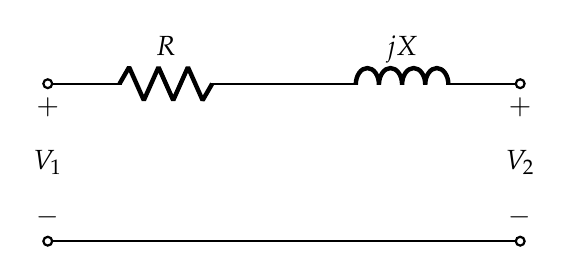
\begin{tikzpicture}
\draw[color=black, thick]
%Input
(0,2) to [open, v^=$V_{1}$, o-o] (0,0){} 
(0,2) to [R, l=$R$] (3,2) to [L, l=$jX$] (6,2) to [open, v=$V_{2}$, o-o] (6,0) -- (0,0){}

;
\end{tikzpicture}
\caption{Circuit diagram of demonstrating power flow from $V_1$ to $V_2$ across impedance $R + jX$.}
\label{fig:droop_circuit}

\end{figure}
\begin{equation}
P = \frac{V_{1}}{R^2 + X^2} \big( R \left( V_{1}-V_{2}\cos{\delta_{12}} \right) +X V_{2} \sin{\delta_{12}} \big)
\end{equation}

Assuming a small phase angle $\delta_{12}$ between the points as well as negligible resistance $R$, the equation can be reduced to 
\begin{equation}
P = \frac{V_1V_2}{X}\delta_{12}
\end{equation}
In practice, the frequency is used rather than the angle because individual units do not know the phase of other units due to the lack of communication. For power and frequency deviation from predefined references the droop equation becomes
\begin{equation}
f = f_{\text{ref}} + K_P\left(P - P_{\text{ref}}\right)
\end{equation}
\nomenclature[V]{$Q$}{Reactive electrical power\nomunit{\si{\voltampreactive}}}
\nomenclature[V]{$f$}{Frequency\nomunit{\si{\hertz}}}
\nomenclature[V]{$V$}{Voltage\nomunit{\si{\volt}}}
where $K_P$ is a negative proportionality constant. 

%\nomenclature[V]{$K_P$}{Negative proportionality constant between change in frequency and change in power in droop control schemes.}


Similarly a droop relationship between reactive power flow and relative voltage levels can be shown:
\begin{equation}
Q = \frac{V_1}{R^2 + X^2} \big( -R V_2 \sin{\delta_{12}} + X \left(V_1 - V_2 \cos{\delta_{12}}\right) \big)
\end{equation}
\begin{equation}
Q = \frac{V_1}{X} \left( V_1 - V_2 \right)
\end{equation}
\begin{equation}
V = V_{\text{ref}} + K_Q \left( Q - Q_{\text{ref}} \right)
\end{equation}
where $K_Q$ is a negative proportionality constant. 

It should be noted, however, that the droop equations are only valid under certain conditions. If the angle\slash frequency deviations are too large then the small angle approximations will break down. Additionally, the relative magnitude of the resistive and reactive impedance components effect system dynamics. If the frequency changes are too large then $X$ can no longer be considered constant. This means the $P$\slash $f$ and $Q$\slash $V$ relationships cannot be approximated as linear. Additionally, the line resistance in most low voltage systems is not so small as to be negligible. In fact in situations where the line reactance is negligible compared to the resistance, linear approximations can be made between active power and voltage as well as reactive power and frequency \cite{YunWeiLi2009}.


%distributed control vs centralized
%droop control vs Master/slave
%Katiraei et al & Vandoorn et al

\section{AC vs DC Microgrids}
AC microgrids and DC microgrids are both technically feasible, but the selection of which is optimal for a given application heavily depends on the types of loads and power sources used. Furthermore, the choice is not necessarily a binary decision. AC\slash DC hybrid systems can provide the benefits of each architecture, but at greater cost. This section will compare and contrast the different architectures.

\subsection{Efficiency}
In each conversion step there is some power loss due to inefficiencies. Sequential conversions can add up to a significant losses. Distributing AC and DC power to their respective loads separately can eliminate many conversion steps but it is unrealistic to completely remove all steps. \autoref{tab:conv_eff} shows that, at rated values, typical losses among different power converters are not symmetric. Transformers are the most efficient, followed by inverters and DC-DC converters. Rectifiers incur the most loss. When operated below rated values all conversion devices experience drops in efficiency.

\begin{table}[]
\centering
\caption{Efficiencies of typical power conversion devices.}
%Keep an eye out for efficiency values more recent the 2006 and 2008
\label{tab:conv_eff}
\begin{tabular}{|ll|l|l|}
\hline
	&				& \multicolumn{1}{l}{From}	&				\\ \cline{3-4} 
	&				& AC				& DC				\\ \hline 
To	& \multicolumn{1}{|l|}{AC}	& 98\% \cite{Starke2008}	& 90\% \cite{Pang2006}	\\ \cline{2-4} 
	& \multicolumn{1}{|l|}{DC}	& 97\% \cite{Starke2008}	& 95\% \cite{Starke2008}	\\ \hline
\end{tabular}
\end{table}
 
% Keep a look out for conversion efficiency more recent than 2006 and 2008

Additionally, distribution power losses are not identical for AC and DC systems. For an AC and DC\footnote{Assuming a DC neutral line introduced.} system, each delivering the same active power and experiencing equal distribution losses, the relationship of RMS current is given as $\frac{I_{AC}}{I_{DC}} = \sqrt{\frac{2}{3}} \approx 0.82$ and a RMS voltage relationship is $\frac{V_{AC}}{2V_{DC}} = \frac{1}{\cos{\theta}} \sqrt{\frac{2}{3}} \approx \frac{0.82}{\cos{\theta}}$ where $\theta$ is the phase angle between $V_{AC}$ and $I_{AC}$ \cite{Starke2008}. Despite the small advantage of DC has over AC in this respect, distribution losses are typically smaller than losses due to conversion.

\subsection{Stability}
Electric machinery and power electronic conversion devices introduce undesired harmonics into AC grids due to non-linear loading effects \cite{Grotzbach1997}. Harmonic distortion can cause power losses as well as reduce voltage and frequency stability. Because harmonics are, by definition, based off of a fundamental frequency the harmonics alone are not an issue in DC segments of a microgrid system. DC systems can experience stability issues caused by non-linear loads such as spikes in current and voltage.

Another important factor in grid stability is how quickly and safely the system can clear an electrical fault. The sinusoidal oscillation of AC systems means there is a periodic zero crossing 60 times each second.\footnote{For regions that operate on 60 Hz.} This means faults can be cleared more quickly in AC systems than in DC systems.  However, AC systems typically experience larger transient spikes during fault events when compared to comparable DC systems \cite{Estes2011}. 

\subsection{Economics}
Most existing electrical infrastructure is built around AC grids rather than DC grids. Furthermore off the shelf electrical appliances generally assume AC power is available and will rectify to DC if needed. These factors indicate the installation of an AC distribution system is more economical. However, AC systems require three lines for each phase, and sometimes a forth neutral line, while DC systems only require two, and sometimes a third neutral line.\footnote{Although work has been done on Single Line Ground Return systems which only require one line.} Although the economic benefit of fewer electrical lines is much more significant to long distance transmission rather than distribution to near by loads.

One benefit of DC microgrids over AC is the necessity to control only voltage level rather than voltage and frequency. A simplified control scheme can reduce the cost combining power sources into a DC bus before distribution avoids the necessity of synchronization \cite{Lotfi2015}.

\section{Thesis Organization}
With the background information on microgrids addressed in \autoref{ch:intro} above, the remainder of the thesis is organized as followed. \autoref{ch:conv} will delve deeper into background of power conversion. This includes the conversion of heat to electricity, with a focus on low-temperature sources, as well electrical power conversion, focusing on the pros and cons of different topologies. 
%\autoref{ch:geothermal} will address necessary background on geothermal power generation. 
\autoref{ch:model} will detail development of the ORC and asynchronous model and its validation. \autoref{ch:analysis} will analyze the simulation results of the greenfield and brownfield scenario.  \autoref{ch:conclusion} will conclude the thesis and describe future work to be conducted on the topic.

\cleardoublepage


\chapter{Energy Conversion}
\label{ch:conv}

Energy and power take many different forms, from the initial sources and to the end results used. Necessarily, methods have been developed to convert the different forms of energy or power from one to another. The first method addressed in this chapter is the conversion of heat to mechanical energy to electrical energy found in heat engines and generators. Next conversion between different forms of electrical power will be addressed.

%This file used to contain the geothermal chapter, now contains thermal/mechanical section of the conversion chapter
\section{Thermal Energy}
Thermal energy, or heat, can originate from many different sources including combustion of a fuel, radioactive decay, or absorption of light from the sun. Heat can be used directly to warm a building, but it is also a critical step in most traditional methods of generating electrical power. 
%\chapter{Geothermal Energy}
%\label{ch:geothermal}

\subsection{Enthalpy}
Enthalpy describes the energy of a system available to be converted to work. It is related to the temperature of the geothermal resource, but also dependent on the pressure and volume. Temperature is usually the primary metric of a geothermal resource, but even a high temperature source is useless without sufficient volume flow. Quantitatively enthalpy is expressed as 
\begin{equation}
H = U + pV
\end{equation}
where $U$ is the internal energy, which is function of temperature, $p$ is the pressure of the system, and $V$ is the volume. Generally it is more convenient to use the change in enthalpy rather than absolute values. After any a system undergoes some thermodynamic process the system will always have some remaining internal energy, pressure, and volume. Therefore a change in enthalpy better describes the energy extracted from (or absorbed by) the system.

Geothermal systems can be classified as high-, medium-, or low-enthalpy\footnote{While the technical definitions differ, the terms enthalpy, heat, and temperature are often used interchangeably when describing geothermal sources.}. Although there is no formal delineation, high-enthalpy sources generally have temperatures greater than about $150$ \textcelsius{} ($302$ \textdegree{}F) and low-enthalpy sources have temperatures lower than $100$ \textcelsius{} ($212$ \textdegree{}F) \cite{Norden2011}. Depending on the amount of extractable energy of the resource, different geothermal processes or cycles should be used.

\subsection{Geothermal Cycles}
%%Describe each of the following but focus on cycles for low enthalpy sources


\subsubsection{Dry Steam}
This high-enthalpy processes extracts hot steam from the earth. The steam is sent directly through a turbine then condensed into liquid water and injected back underground. 

\subsubsection{Flash Steam} 
In the flash steam process high pressure hot is water extracted then allowed to boil becoming steam and low pressure hot water. The steam is sent through a turbine then condensed, recombined with water, and injected back underground.

\subsubsection{Binary Cycle} 
As the name implies, binary cycles involve two loops: a heat source loop and working fluid loop. Heat is collected in the heat source loop and transferred to the working loop through a heat exchanger. The working fluid then undergoes the vaporization process to spin a turbine or screw expander. Binary cycles are technically not limited to low- or medium-enthalpy resources, however high-enthalpy system can be implemented directly with a single loop using the flash or dry steam processes. The most common binary cycle is the Organic Rankine Cycle (ORC) which uses an organic working fluid such as refrigerants. Working fluids are selected for low vaporization temperatures relative to water.

%\subsubsection{(Organic) Rankine Cycle}
%\subsubsection{Kalina Cycle}

\subsection{Synchronous and Asynchronous Generators}
%This section should focus the difference between the two with respect to geothermal sources. I can have a fundemental description of the generators either in this chapter or the intro chapter.

%Direct drives

%\subsection{Pilgrim Hot Springs}
%More thourough description of the resource and potential development plans.

\subsection{ORC Manufacturers and Developers}
\subsubsection{Under Development}
\begin{description}
\item[Air Squared]
\item[Termo2Power]
\item[Climeon]
\item[Calnetix/Access Energy]
\item[Verdicorp] has a range of variable speed expanders. The expander connects to the rotor of a permanent magnet synchronous generator. An IGBT variable frequency drive converts and synchronizes the power with a local grid.
\item[Inifinity Turbine]
\item[Ener-G-Rotors]
\item[Phoenix]
\end{description}
\subsubsection{Commercial Products}
\begin{description}
\item[Electratherm] makes use of a twin screw expander to spin an induction generator.
\item[E-Rationale] uses a single screw expander to rotate an induction generator.
\item[Exergy] %radial outflow turbine
\item[Zuccato] uses a radial inflow turbine directly connected to synchronous permanent magnet generator. Electric power is converted and synchronized to local power grid with IGBT switching.
\item[Enogia] uses a turboexpander. Electric power is rectified then tied into the grid with a grid feed inverter.
\item[Clean Energy Technologies] %uses high speed turbine 
\item[Tri-O-Gen] %uses high speed turbine 
\end{description}
 %used to contain geothermal chapter, now contains thermal section

\section{Electric Conversion}

\subsection{Linear Power Supplies}
%Linear

\subsection{Switched Mode Power Supplies}

\subsection{PWM vs PFM}

\subsection{DC-DC}
recent developments

\subsection{Rectifiers}
recent developments

\subsection{Inverters}
recent developments

%%This file used to contain the geothermal chapter, now contains thermal/mechanical section of the conversion chapter
\section{Thermal Energy}
Thermal energy, or heat, can originate from many different sources including combustion of a fuel, radioactive decay, or absorption of light from the sun. Heat can be used directly to warm a building, but it is also a critical step in most traditional methods of generating electrical power. 
%\chapter{Geothermal Energy}
%\label{ch:geothermal}

\subsection{Enthalpy}
Enthalpy describes the energy of a system available to be converted to work. It is related to the temperature of the geothermal resource, but also dependent on the pressure and volume. Temperature is usually the primary metric of a geothermal resource, but even a high temperature source is useless without sufficient volume flow. Quantitatively enthalpy is expressed as 
\begin{equation}
H = U + pV
\end{equation}
where $U$ is the internal energy, which is function of temperature, $p$ is the pressure of the system, and $V$ is the volume. Generally it is more convenient to use the change in enthalpy rather than absolute values. After any a system undergoes some thermodynamic process the system will always have some remaining internal energy, pressure, and volume. Therefore a change in enthalpy better describes the energy extracted from (or absorbed by) the system.

Geothermal systems can be classified as high-, medium-, or low-enthalpy\footnote{While the technical definitions differ, the terms enthalpy, heat, and temperature are often used interchangeably when describing geothermal sources.}. Although there is no formal delineation, high-enthalpy sources generally have temperatures greater than about $150$ \textcelsius{} ($302$ \textdegree{}F) and low-enthalpy sources have temperatures lower than $100$ \textcelsius{} ($212$ \textdegree{}F) \cite{Norden2011}. Depending on the amount of extractable energy of the resource, different geothermal processes or cycles should be used.

\subsection{Geothermal Cycles}
%%Describe each of the following but focus on cycles for low enthalpy sources


\subsubsection{Dry Steam}
This high-enthalpy processes extracts hot steam from the earth. The steam is sent directly through a turbine then condensed into liquid water and injected back underground. 

\subsubsection{Flash Steam} 
In the flash steam process high pressure hot is water extracted then allowed to boil becoming steam and low pressure hot water. The steam is sent through a turbine then condensed, recombined with water, and injected back underground.

\subsubsection{Binary Cycle} 
As the name implies, binary cycles involve two loops: a heat source loop and working fluid loop. Heat is collected in the heat source loop and transferred to the working loop through a heat exchanger. The working fluid then undergoes the vaporization process to spin a turbine or screw expander. Binary cycles are technically not limited to low- or medium-enthalpy resources, however high-enthalpy system can be implemented directly with a single loop using the flash or dry steam processes. The most common binary cycle is the Organic Rankine Cycle (ORC) which uses an organic working fluid such as refrigerants. Working fluids are selected for low vaporization temperatures relative to water.

%\subsubsection{(Organic) Rankine Cycle}
%\subsubsection{Kalina Cycle}

\subsection{Synchronous and Asynchronous Generators}
%This section should focus the difference between the two with respect to geothermal sources. I can have a fundemental description of the generators either in this chapter or the intro chapter.

%Direct drives

%\subsection{Pilgrim Hot Springs}
%More thourough description of the resource and potential development plans.

\subsection{ORC Manufacturers and Developers}
\subsubsection{Under Development}
\begin{description}
\item[Air Squared]
\item[Termo2Power]
\item[Climeon]
\item[Calnetix/Access Energy]
\item[Verdicorp] has a range of variable speed expanders. The expander connects to the rotor of a permanent magnet synchronous generator. An IGBT variable frequency drive converts and synchronizes the power with a local grid.
\item[Inifinity Turbine]
\item[Ener-G-Rotors]
\item[Phoenix]
\end{description}
\subsubsection{Commercial Products}
\begin{description}
\item[Electratherm] makes use of a twin screw expander to spin an induction generator.
\item[E-Rationale] uses a single screw expander to rotate an induction generator.
\item[Exergy] %radial outflow turbine
\item[Zuccato] uses a radial inflow turbine directly connected to synchronous permanent magnet generator. Electric power is converted and synchronized to local power grid with IGBT switching.
\item[Enogia] uses a turboexpander. Electric power is rectified then tied into the grid with a grid feed inverter.
\item[Clean Energy Technologies] %uses high speed turbine 
\item[Tri-O-Gen] %uses high speed turbine 
\end{description}
	%Electronic conversion and thermal/mechanical conversion chapters combined
\chapter{Model Description}
\label{ch:model}

The model attempts to recreate a microgrid which uses some form of DER as a primary power source along side energy storage in order power the load. \autoref{fig:abridged_flow_diagram} shows a simplified flow diagram of the model using an ORC for the DER. The components include a ORC as a source, a load, and an inverter to link the source two. In the figure, the blue lines represent electrical connections, while green represents the flow of data and component parameters. The ORC block is made up of heat exchangers, an isentropic pump, an isentropic expander, and an induction generator. 
\begin{comment}
The load block \verb|one line description of load|. 
The energy storage block \verb|one line description of energy storage|. 
The inverter block \verb|one line description of inverter|.
\end{comment}
\begin{figure}[ht]
	\centering
	\caption{A simplified diagram of power and data flows of the model. Blue lines represent electrical power connections and flows similar to a one-line diagram. Green boxes data flow from one part of the model to another.}
	\label{fig:abridged_flow_diagram}
	
	%\includegraphics[width=\textwidth]{figures/Abridged Pilgrim Model Flow diagram - AC bus.pdf} 
	\includegraphics[width=\textwidth]{figures/SimpleFlowDiagram.pdf}

\end{figure}

\section{Organic Rankine Cycle Generator}
The ORC generator block links the thermal, mechanical, and electric components of them model. The thermal properties of the fluids were obtained from a Matlab wrapper of the CoolProp library. \cite{Bell2014} Thermal conditions of source, sink, and working fluids are fed into the Rankine Cycle portion of the model, which returns a mechanical power. Electrical conditions, along with the mechanical power, are fed into the generator portion of the model, which returns an electrical output.  

\subsection{Evaporator and Condenser}
The evaporator and the condenser are both represented using a heat exchanger script.  The function takes as inputs parameters about the high and low temperature fluids, specifically the inlet temperatures or enthalpies ($\si{\kelvin}$ or $\si{\joule\per\kilogram}$), mass flow rates ($\si{\kilogram\per\second} $), inlet pressures ($\si{\pascal}$), and fluid names, as well as parameters about the exchanger itself such as the overall heat transfer coefficient ($\si{\watt\per\kelvin\per\meter\squared}$), the heat transfer area ($\si{\meter\squared}$), and the heat exchanger type (e.g. counter or parallel flow). The function output is made up of the heat flow rate ($\si{\watt}$), and the temperatures or enthalpies at the outlets ($\si{\kelvin}$ or $\si{\joule\per\kilogram}$). 

In order to calculate the desired values, the Number of Transfer Units (NTU) method is used. Described in The Fundamentals of Heat and Mass Transfer, \cite{Incropera} this process calculates the output heat flow, $\dot{Q}$, relative to a theoretical maximum heat flow, $\dot{Q}_{max}$. This potential heat flow would be realized using an infinitely long counter flow geometry and is calculated as
\begin{equation}
\dot{Q}_{max} = C_{min}\left(T_{h,i} - T_{c,i}\right)
\end{equation}
where $C_{min}$ is the smaller heat capacity rate of the hot and cool fluids and $T_{h,i}$ and $T_{c,i}$ are the inlet temperatures of hot and cool fluids respectively. The heat capacity rate is the product of mass flow rate, $ \dot{m} $, and the mass specific heat at constant pressure, $ c_p $. 

The heat flow rates of the hot and cool fluids are related by the effectiveness, $\epsilon$, which is defined as 
\begin{equation}
\label{eq:effectiveness_def}
\epsilon \equiv \frac{\dot{Q}}{\dot{Q}_{max}}
\end{equation}

Numerically, the value of $\epsilon$ is a function of the ratio of the fluids' heat capacities, $C_r = \frac{C_{min}}{C_{max}}$, as well as the exchanger's Number of Transfer Units, $NTU = \frac{U \cdot A}{C_{min}}$, where $U$ is the overall heat transfer coefficient and $A$ is the total heat transfer area. Additionally, the direction of fluid flow changes the method of calculation. In parallel flow heat exchangers, the effectiveness is calculated as
\begin{equation}
\epsilon = \frac{1 - \exp\left[-NTU\left(1 + C_r\right)\right]}{1 + C_r}
\end{equation}
while counter flow devices use
\begin{equation}
\epsilon = \frac{1 - \exp\left[-NTU\left(1 - C_r\right)\right]}{1 - C_r\exp\left[-NTU\left(1 - C_r\right)\right]}
\end{equation}

Once the effectiveness and maximum heat transfer rate are determined, equation \ref{eq:effectiveness_def} is used to calculate the actual rate of heat flow, $\dot{Q}$. Finally, the change in temperature for each fluid is calculated based on their respective heat capacity rates at initial conditions and the rate of heat flowing between them. 
If the change in temperature for either fluid would result in vaporization or condensation, then the values must be recalculated because the specific heat is effectively infinite while the fluid is changing states. 

First, the heat flow rate necessary to have the fluid begin changing its state is determined and the fraction of this value relative to initial heat flow rate is calculated. 
The heat transfer area is reduced by this fraction and the function is re-run inputing the state of the two fluids as the one fluid begins to change phase. If enough heat flows between the two fluids such that the one completes the phase change, then the function is run a third time with the heat transfer area modified again. 

Within this script there are certain assumptions made in order to calculate the output values. The function will not return accurate results if both fluids simultaneously undergo a phase change because the ratio of heat capacities, $C_r$, will be undefined. Additionally, Ambient temperature and associated heat flow to the external environment is not accounted for in the script. Finally, it is assumed the pressure drop from inlet to outlet is negligible for both the high and low temperature fluids. 

\subsection{Expander and Pump}
The expander/turbine and pump components are both modeled by a fluid undergoing non-ideal isentropic expansion or compression. For an ideal isentropic process, the fluid will experience some thermodynamic changes while its internal entropy remains constant. 

The function takes as inputs certain properties of the fluid, such as the inlet temperature or enthalpy ($\si{\kelvin}$ or $\si{\joule\per\kilogram}$), both the inlet and outlet pressures ($\si{\pascal}$), and the mass flow rate ($\si{\kilogram\per\second}$). Also needed is the isentropic efficiency, a unitless parameter of the machine which describes lost power due to deviations from the ideal insentropic process. The function returns the power produced or consumed\footnote{Power is produced if the pressure at the inlet is greater than at the outlet, and consumed if inlet pressure is less than that of the outlet.} ($\si{\watt}$) and the temperature or enthalpy ($\si{\kelvin}$ or $\si{\joule\per\kilogram}$) of the fluid at the outlet.

Using the inputs and the Cool Prop library, the Mass Specific Entropy, $S$, of the fluid is determined for the fluid at the inlet. In an ideal process, this value would remain constant, so it is used to determine the ideal enthalpy of the outlet. Next the ideal power transferred is calculated as 
\begin{equation}
\label{eq:power_enthalpy}
P = \dot{m} \left(H_i - H_o\right)
\end{equation}
where $H_i$ and $H_o$ are the inlet and outlet enthalpies respectively.

To obtain the actual transfered power, the isentropic efficiency is applied to the ideal power such that the ideal is necessarily greater than the actual. When the value of $H_i$ is larger than $H_o$, $P$ is positive\footnote{Power is produced.} therefore efficiency is multiplied. When $H_i$ is less than $H_o$, $P$ is negative\footnote{Power is consumed.} and ideal power is divided by efficiency. After actual transferred power is calculated, equation \ref{eq:power_enthalpy} is used to find $H_o$ and the fluid temperature at the outlet.

\subsection{Induction Generator}
The generator block models a Squirrel Cage Induction Generator (SCIG) in order to convert the mechanical power to an electrical form. Two different function blocks were created for two scenarios: regulated and unregulated. The former is simpler to model, but the generator requires another firm source\footnote{Or an electrical storage-inverter combination.} to maintain its frequency and voltage. For the latter scenario, the generator's frequency and voltage are allowed to vary. Its leads are connected directly to a power converter which maintains the frequency and voltage of the remaining microgrid. 

\subsubsection{Regulated SCIG}
This function block takes several electrical and mechanical parameters as inputs such as the line to line voltage ($\si{\volt}$) and electrical frequency ($\si{\hertz}$) at the leads, the mechanical speed at the shaft ($\si{\rpm}$), the number pole pairs in machine's windings, and coefficients of friction due to bearings ($\si{\watt\per\second}$) and windage ($\si{\watt\per\second\squared}$). Also input are the resistive and inductive impedances ($\si{\ohm}$) of the stator, rotor, and core, as well as the capacitive impedance and equivalent series resistance of external excitation capacitor. The function returns the active ($\si{\watt}$) and reactive ($\si{\voltampreactive}$) power outputs and losses.

\begin{figure}[h]
	
\centering

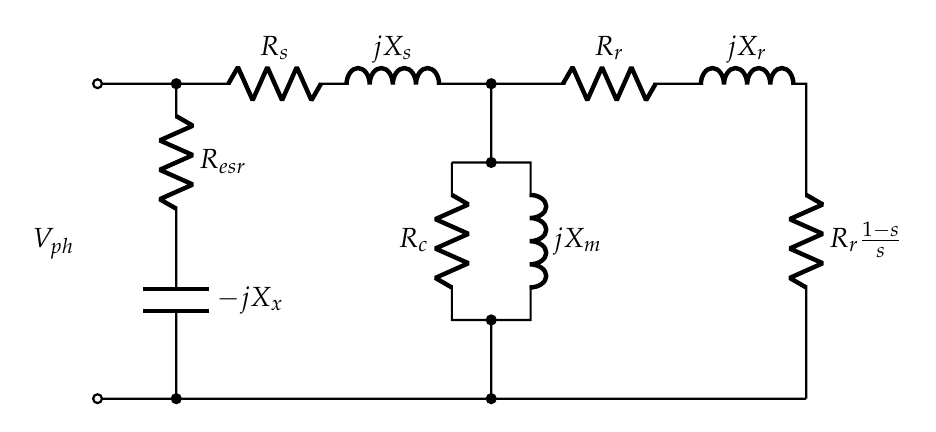
\begin{tikzpicture}[american voltages]
\draw[color=black, thick]
%Input
(0,0) to [open, l=$V_{ph}$, o-o] (0,4){}

%low
(0,0) -- (9,0){}

%stator
(0,4) -- (1.5,4) to [R, l=$R_{s}$] (3,4) to [L, l = $j X_{s}$] (4.5,4){}

%rotor
(4.5,4) -- (5.5,4) to [R, l=$R_{r}$] (7.5,4) to [L, l = $j X_{r}$] (9,4) to [R, l=$R_{r}\frac{1-s}{s}$] (9,0){}

%core
(5,4) to [short, *-*] (5,3){}
(4.5,3) -- (5.5,3) to [L, l = $j X_{m}$] (5.5,1) -- (4.5,1) to [R, l=$R_{c}$] (4.5,3){}
(5,1) to [short, *-*] (5,0){}

%external excitaion capacitor
(1,4) to [R, l=$R_{esr}$, *-] (1,2) to [C, l=$-j X_x$] (1,0.5) to [short, -*] (1,0){}


;
\end{tikzpicture}

\caption{Single phase diagram of a three phase squirrel cage induction machine. $V_{ph}$ and $s$ are the phase voltage and slip of the generator. }
\label{fig:SCIG__circuit_diagram}

\end{figure}
A single phase circuit diagram of the generator which includes these components can be seen in \autoref{fig:SCIG__circuit_diagram}. $R_s$ and $X_s$ represent the resistive and inductive impedances of the stator. $R_r$ and $X_r$ represent the resistive and inductive impedances of the rotor as referred to the stator. $R_c$ and $X_m$ represent the resistive and inductive impedances due to the magnetization of the core. $R_{esr}$ and $X_x$ represent the equivalent series resistance and capacitive impedances of the external excitation capacitor.

To calculate these outputs, first the magnitude of the phase voltage is determined from the line to line voltage, $V_{ll}$, as $ \left|V_{ph}\right| = \frac{\left|V_{ll}\right|}{\sqrt{3}} $ assuming $ \angle V_{ph} = 0\deg $. Next the synchronous mechanical speed is determined by $ n_{synch} = \frac{120f}{2\text{poles}} $ and is used, along with the mechanical speed, $n_{mech}$ to calculate the slip of the machine as $ s = \frac{n_{synch} - n_{mech}}{n_{synch}} $.

The impedances of the stator, rotor, core impedances, the Th\'evenin combination of those three branches, the external excitation branch, and the Th\'evenin combination of all branches are calculated as
\begin{equation*}
Z_s = R_s + jX_s
\end{equation*}
\begin{equation*}
Z_r = R_r\frac{1-s}{s} + R_r + jX_r
\end{equation*}
\begin{equation*}
Z_{core} = R_c \parallel jX_m
\end{equation*}
\begin{equation*}
Z_{machine} = R_s + \left(Z_{core} \parallel Z_r\right)
\end{equation*}
\begin{equation*}
Z_{excite} = R_{esr} - jX_x
\end{equation*}
\begin{equation*}
Z_{total} = Z_{excite} \parallel Z_{machine}
\end{equation*}

Once all the relevant impedances are determined, the currents flowing through the branches are calculated along with the internal voltage at the stator-rotor-core junction. These values are used to determine internal power losses. The mechanical losses due to the bearings and windage are calculated by multiplying the appropriate coefficient of friction by the mechanical angular frequency  and the square of the mechanical angular frequency respectively. 

\subsubsection{Unregulated SCIG}
To simulate microgrids with no forms of storage or sources beyond the ORC, an unregulated SCIG model was developed. The single phase diagram is similar to the regulated SCIG seen in \autoref{fig:SCIG__circuit_diagram}, except the voltage source $V_{ph}$ at the lead is replaced with a resistive load. The model is based off the analysis by Ouazenne et al. of a self excited induction generator in \cite{Ouazenne1983} using admittance balancing. It is assumed the active power losses across the core and the excitation capacitance are negligible. Additionally, it is assumed the load is purely active, as any reactive load can be supplied by the conversion device which regulates the voltage and frequency of the microgrid.

The method of admittance balancing relies on the fact active and reactive power entering and exiting an electrical node must sum to zero. For this analysis, the chosen node at which the rotor, the core, and the combination of the stator, excitation capacitor, and load meet. Since the voltage across each branch is the same and power flow sums to zero, then the admittances must sum to zero as well. By breaking the complex admittances into real and imaginary components, a system of equations can be developed to solve for frequency and core reactance. A more detailed description of this process can be seen in Appendix \autoref{ap:SEIG}. These values can then be used to determine total power output and losses. 

The function takes as variable inputs the mechanical speed of the shaft ($\si{\rpm}$), the power load of the microgrid ($\si{\watt}$), and the line to line voltage at the lead ($\si{\volt}$). Also input as parameters are the rated frequency of machine ($\si{\hertz}$), the number of poles it contains, the resistances and inductances of the rotor and stator ($\si{\ohm}, \si{\henry}$), the capacitance of external excitation capacitors ($\si{\farad}$), coefficients of friction due to bearings ($\si{\watt\per\second}$) and windage ($\si{\watt\per\second\squared}$), and the magnetization curve comparing the core reactance ($\si{\ohm}$) to the internal voltage across the core ($\si{\volt}$). The output variables of the function include active power generated ($\si{\watt}$) and internally consumed ($\si{\watt}$), the reactive power consumed ($\si{\voltampreactive}$), the necessary mechanical power driving the shaft ($\si{\watt}$), the line to line voltage ($\si{\volt}$), and the electrical frequency ($\si{\hertz}$).

First the inductive and capacitive reactances of the rotor, stator, and external excitation capacitors are calculated at the rated frequency of the machine, along with the equivalent load resistance for the given input voltage. Next, the electrical frequency is calculated based off the real portion of the admittance balance equations. With the frequency the machine slip can be determined as well. Next, the imaginary portion of the admittance balance equation can be used to solve for the core reactance. Internal voltage of the machine is then interpolated from the core reactance based off of the magnetization curves. The new line voltage is determined as well to feed back into the next iteration of the function.

With all components of the machine known, the power output and losses can be calculated in the same manner as the regulated induction generator seen above. The power generated is fed into the input of the inverter block and the losses are used in the feedback control.

\section{Inverter}
The inverter block converts the unregulated power output from the generator into a form with a stable frequency and voltage. In this model, a simplified view is taken of its operation. The inputs include the inverter's efficiency, $\eta$, and the unregulated power off of the induction generator ($\si{\watt}$). The outputs include the delivered power to the load calculated as $P_{out} = \eta P_{in}$  and the power lost within the inverter ($\si{\watt}$) calculated as $P_{loss} = P_{in} - P_{out}$. 

\section{Load}
The model is assumes the microgrid delivers power to a three-phase $\SI{60}{\hertz}$ AC load. The total load in the model is determined by the sum of a predefined set point and the power consumed by the pump used to circulate the working fluid. In addition to the active load, it is assumed there is a reactive load determined by a predefined power factor parameter. 
The load seen by the unregulated induction generator is the sum of the total load and the losses due to the inverter. 

The total load is combined with both the inverter and generator losses in order to provide the reference of a PI controller. The sum is then compared to the output mechanical power of the ORC system. A gain is applied to the error signal and integrated to provide the desired flow rate of the working fluid. The gain value was selected in order to quickly reach steady state during the simulation.


\chapter{ORC System Model Validation, Analysis, and Case Study Results}
\label{ch:analysis}

With the ORC prime power system model constructed as described in \autoref{ch:model}, simulations were conducted to validate and verify the model. After validation, two case studies, a greenfield and brownfield microgrid, were investigated and analyzed in order to determine whether geothermal ORC generators can be viably used as primary power sources.

\section{Validation}
%Before simulating  the greenfield and brown field case study scenarios, the model needs to be validated. 
The model validation is conducted by comparing the results of an ORC test with the simulation results under similar conditions. The test, performed in 2013, is from the University of Alaska Fairbanks and is documented in a report by Lin et al. \cite{Lin2014}. The report details the process of testing an Electratherm Green Machine ORC system in a controlled environment at the UAF power plant.
%and in the field for waste heat reclamation of a diesel generator at the Tok, Alaska powerhouse.

During the sizing of the ORC system, turbine and pump efficiencies, 
$\eta_{turbine}$ and $\eta_{pump}$, as well as heat exchanger areas, $A_{evap}$ and $A_{cond}$, and transfer coefficients, $U_{evap}$ and $U_{cond}$, were assumed based off of published values and conventional practice, but final values were not reported. These assumed values are used as the input to the model. All of the non-variable ORC prime power system parameters used for the model validation can be seen in \autoref{tab:verification_ORC_params}.
\begin{table}%[h]
	\centering
	\caption{Input parameters for the validation of the ORC prime power system model.}
	%\rowcolors{5}{}{gray!10}
	\label{tab:verification_ORC_params}
	\begin{tabular}{rl}
		\toprule
		           Parameter & Value                                        \\ \midrule
		         $U_{evap}$ & 1500 \si{\watt\per\kelvin\per\meter\squared} \\
		         $A_{evap}$ & 26.5 \si{\meter\squared}                     \\
		         $U_{cond}$ & 1400 \si{\watt\per\kelvin\per\meter\squared} \\
		         $A_{cond}$ & 102.5 \si{\meter\squared}                    \\
		    $\eta_{turbine}$ & 0.78                                         \\
		       $\eta_{pump}$ & 0.7                                          \\
		$\eta_{pump\ driver}$ & 0.9                                          \\
		   $\eta_{inverter}$ & 1.0                                          \\ \bottomrule
	\end{tabular}
\end{table}


The only reported electrical parameters of the three phase induction generator were the frequency (\SI{60}{\hertz}) and the line to line voltage (\SI{480}{\volt}AC). The impedance parameters were taken from a 10 HP machine in \cite{Ouazenne1983} and scaled based off the expected relative power output. The external excitation capacitance, $C_x$, was selected in order to yield a terminal voltage roughly equal to the rated voltage. The impedance parameters can be seen in \autoref{tab:verification_SCIG_params}.
% and the magnetization curve comparing internal voltage, $E$, and the magnetizing reactance at rated frequency, $X_m$, can be seen in Fig X.
\begin{table}%[h]
	\centering
	\caption{Input generator parameters for the verification of the Organic Rankine Cycle model.}
	%\rowcolors{5}{}{gray!10}
	\label{tab:verification_SCIG_params}
	\begin{tabular}{rl}
		\toprule
		    Parameter & Value                                       \\ \midrule
		      $poles$ & 4                                           \\
		  $f_{rated}$ & $\SI{60}{\hertz}$                           \\
		        $R_s$ & $\SI{0.0279}{\ohm}$                         \\
		        $X_s$ & $\SI{0.0798}{\ohm}$                         \\
		        $R_r$ & $\SI{0.0272}{\ohm}$                         \\
		        $X_r$ & $\SI{0.0475}{\ohm}$                         \\
		        $C_x$ & $\SI{1000}{\micro\farad}$                   \\
		    $R_{esr}$ & $\SI{0}{\ohm}$                              \\
		 $K_{bering}$ & $\SI{0.5}{\kilo\watt\per\second}$           \\
		$K_{windage}$ & $\SI{0.003}{\kilo\watt\per\second\squared}$ \\ \bottomrule
	\end{tabular}
\end{table}

%\input{figures/magCurve}

Four loads were simulated under different combinations of heat sink flow rates and heat source temperatures and flow rates, as well as high and low pressure values as shown in  \autoref{tab:verification_ORC_vars}. For the validation process pressure values used based on estimates within reported pressure ranges. The working fluid flow rate was also not reported, and therefore could not be used as an input to the model. Instead the model uses load power set points such that the gross power produced by the simulation approximately matches the reported value and returns the necessary working fluid flow rate to achieve that power output.  
\begin{table}[h]
	\centering
	\caption{Input variables for the verification of the Organic Rankine Cycle Model.}
	%\rowcolors{5}{}{gray!10}
	\label{tab:verification_ORC_vars}
	\begin{tabular}{rllll}
		\toprule
		                                              &  Case &       &       &       \\ \cline{2-5}
		                                              &     1 &     2 &     3 &     4 \\ \midrule
		$T_{source,in}(\si{\kelvin})$                 & 363.9 & 363.6 & 353.0 & 363.9 \\
		$T_{sink,in}(\si{\kelvin})$                   & 283.5 & 284.6 & 283.6 & 284.6 \\
		$\dot{m}_{source}(\si{\kilogram\per\second})$ &  18.3 &  7.28 &  18.4 &  7.35 \\
		$\dot{m}_{sink}(\si{\kilogram\per\second})$   &  13.0 &  7.53 &  13.0 &  7.54 \\
		$p_{hi}(\si{\kilo\pascal})  $                 &  0.68 &  0.75 &  0.60 &  0.60 \\
		$p_{low}(\si{\kilo\pascal}) $                 &  0.14 &  0.17 &  0.14 &  0.16 \\
%		$P_{setpoint}(\si{\kilo\watt})$               &  34.7 &  27.1 &  24.6 &  19.0 \\ 
		\bottomrule
	\end{tabular}
\end{table}



The mechanical power, $P_{mech}$, the generator power, $P_{gen}$, inverter output power, $P_{out}$, and the electrical power consumed by the pump, $P_{pump}$, of the four tests are plotted in \autoref{fig:verificationPower01}. \input{figures/VerificationPower01} 
\autoref{fig:verificationHeat01} \begin{figure}[p]
	\centering
	
	\includegraphics[width=\textwidth]{figures/VerificationHeat01}
	%\includegraphics[width=0.5\textwidth]{figures/VerificationHeat01}
	
	\caption{Comparison of evaporator and condenser heat flow rates for the validation of the ORC prime power system model. All tests assume a sink temperature of \SI{283}{\kelvin} (\SI{10}{\degreeCelsius}). Tests 1 and 2 use a heat source temperature of \SI{364}{\kelvin} (\SI{91}{\degreeCelsius}), while tests 3 and 4 use \SI{353}{\kelvin} (\SI{79}{\degreeCelsius}). Tests 1 and 3 use a source flow rate of \SI{19}{\liter\per\second} and a sink flow rate of \SI{13}{\liter\per\second}, where as tests 3 and 4 use a source and sink flow rate of \SI{8}{\liter\per\second}.
	%The power setpoints of the four tests are \SIlist{27.5;40.0;30.8;42.0}{\kilo\watt}. Tests 1 and 3 use the maximum power setpoint while also ensuring the working fluid fully evaporates in the evaporator. Tests 2 and 4, use the maximum power setpoint while maintaining a stable simulation. 
	}
	%Psetpoint[2.75e4;4.0e4;3.08e4;4.2e4;]
	\label{fig:verificationHeat01}
\end{figure} 
plots the heat flows though the evaporator, $\dot{Q}_{evap}$, and condenser,  $\dot{Q}_{cond}$. The inlet and outlet temperatures of the source, $T_{source\ in}$ and $T_{source\ out}$, and sink, $T_{sink\ in}$ and $T_{sink\ out}$, are plotted in \autoref{fig:verificationWaterTemp01}. \input{figures/VerificationWaterTemp01} 
\autoref{tab:verification_results01} compares simulated values in the plots with the measured values from the report.
\begin{table}%[h]
	\centering
	\caption{Comparison of output variables for the verification of the ORC Model.}
	%\rowcolors{5}{}{gray!10}
	\label{tab:verification_results01}
	\begin{tabular}{rllllllll}
		\toprule
		                                      & Case  &       &       &       &       &       &       &         \\ \cline{2-9}
		                                      & 1     &       & 2     &       & 3     &       & 4     &         \\
		                                      & Meas. & Model & Meas. & Model & Meas. & Model & Meas. & Model   \\ \midrule
		         $P_{gross}(\si{\kilo\watt})$ & 40.7  & 40.6  & 31.8  & 31.6  & 29.2  & 29.2  & 22.7  & 23.0    \\
		          $P_{pump}(\si{\kilo\watt})$ & 2.6   & 4.9   & 1.9   & 5.6   & 1.5   & 4.1   & 1.3   & 4.2     \\
		   %$P_{source pump}(\si{\kilo\watt})$ & 9.6   & -     & 1.0   & -     & 10.0  & -     & 1.0   & -       \\
		     %$P_{sink pump}(\si{\kilo\watt})$ & 3.5   & -     & 1.0   & -     & 3.5   & -     & 1.0   & -       \\
		  $P_{evap.}(\si{\kilo\watt})$ & 519   & 621   & 413   & 540   & 393   & 540   & 328   & 466     \\
		  $P_{cond/}(\si{\kilo\watt})$ & 464   & 583   & 385   & 512   & 356   & 514   & 303   & 446     \\
		       $T_{source,out}(\si{\kelvin})$ & 357.2 & 355.8 & 350.1 & 345.9 & 347.9 & 346.0 & 342.0 & 337.5   \\
		         $T_{sink,out}(\si{\kelvin})$ & 292.1 & 294.2 & 296.9 & 300.9 & 290.1 & 293.0 & 294.2 & 298.7   \\ \bottomrule
		      %$P_{setpoint}(\si{\kilo\watt})$ &       &       &       &       &       &       &       &         \\
    %$\dot{m}_{wf}(\si{\kilogram\per\second})$ & -     &       & -     &       & -     &       & -     &         \\ 
\end{tabular}
\end{table}



As desired, the gross electrical power output of the model matches the measured value for each set of inputs. However, the power consumed to run the pump is a factor of 2-3 times greater in the model than what was measured. A pump sizing guide \cite{CheGuide2017} was used to calculate hypothetical hydraulic power needed to move a liquid at the density of R245-fa across each of the pressure differences listed at the corresponding flow rates. When these hydraulic power values have the assumed pump and drive efficiencies applied as well, they match the pump power values of the model. This indicates the working fluid flow rates of the model are much greater than the operating values measured during the Green Machine ORC system test.

The calculated heat transferred in both the evaporator and the condenser are greater than what was measured in each case. Although the values do tend to follow a similar pattern with higher source temperatures and water flow rates resulting in greater rates of heat transferred. Additionally, the source and sink fluids undergo a greater temperature change in the model as a result of the higher heat flow rates.


%The likely reason for the difference in heat flows is model assumes all the heat flows from one fluid to another and does not affect the ambient temperature. This is also a possible explanation for higher pump power consumptions seen in the model. With both more heat being added and removed from the working fluid, but the same amount of mechanical power being extracted from it, the fluid is likely being 

Pressure was plotted against enthalpy at various points of the cycle in \autoref{fig:verifcation_ph01} \input{figures/verificationPH01} for each of the four tests. The two curves indicate the pressure-enthalpy combinations of R245-fa where the working fluid begins to condense and vaporize. The top-left group of points represents the working fluid state at the outlet of the pump. The top-right group represents the working fluid state at the inlet of the expander. The bottom-right group represents the working fluid state at the outlet of the expander. Finally, he bottom-left group represents the working fluid state at the inlet of the pump.
%\input{figures/verificationPH01}

For each of these tests, the working fluid just barely begins to boil in the evaporator, if at all. It is expected that the working fluid will either completely vaporize, or at least be further to the right in the liquid-vapor region. Along with the higher than expected pump power, this also indicates that there is more working fluid being pumped throughout the cycle in the model than what was measured.

To re-create conditions where the system outputs are comparable between the modeled and measured values while pumping less fluid, the evaporator area is increased by a factor of four so it is comparable to the area of the condenser. Additionally, the pressure set points are adjusted to values seen in \autoref{tab:verification_ORC_vars02} to account for the new temperatures of the working fluid.
\begin{table}%[h]
	\centering
	\caption{Input variables for the verification of the Organic Rankine Cycle Model.}
	%\rowcolors{5}{}{gray!10}
	\label{tab:verification_ORC_vars02}
	\begin{tabular}{rllll}
		\toprule
		                                              &  Case &       &       &       \\ \cline{2-5}
		                                              &     1 &     2 &     3 &     4 \\ \midrule

		$p_{hi}(\si{\kilo\pascal})  $                 &  0.68 &  0.75 &  0.60 &  0.60 \\
		$p_{low}(\si{\kilo\pascal}) $                 &  0.14 &  0.17 &  0.14 &  0.16 \\
%		$P_{setpoint}(\si{\kilo\watt})$               &  34.7 &  27.1 &  24.6 &  19.0 \\ 
		\bottomrule
	\end{tabular}
\end{table}



The results of the second set of validation tests are plotted in \autoref{fig:verificationPower02} \input{figures/VerificationPower02}
for the power values, \autoref{fig:verificationHeat02} \begin{figure}[h]
	\centering
	
	\includegraphics[width=\textwidth]{figures/VerificationHeat02}
	%\includegraphics[width=0.5\textwidth]{figures/VerificationHeat02}
	
	\caption{Comparison of evaporator and condenser heat flow rates for the validation of the ORC prime power system model with an increased evaporator area. All tests assume a sink temperature of \SI{283}{\kelvin} (\SI{10}{\degreeCelsius}). Tests 1 \& 2 use a heat source temperature of \SI{364}{\kelvin} (\SI{91}{\degreeCelsius}), while tests 3 \& 4 use \SI{353}{\kelvin} (\SI{79}{\degreeCelsius}). Tests 1 \& 3 use a source flow rate of \SI{19}{\liter\per\second} and a sink flow rate of \SI{13}{\liter\per\second}, where as test 3 \& 4 use a source and sink flow rate of \SI{8}{\liter\per\second}.
	%The power setpoints of the four tests are \SIlist{27.5;40.0;30.8;42.0}{\kilo\watt}. Tests 1 \& 3 use the maximum power setpoint while also ensuring the working fluid fully evaporates in the evaporator. Tests 2 \& 4, use the maximum power setpoint while maintaining a stable simulation. 
	}
	%Psetpoint[2.75e4;4.0e4;3.08e4;4.2e4;]
	\label{fig:verificationHeat02}
\end{figure} 
for the heat flow rate values, and \autoref{fig:verificationWaterTemp02} \input{figures/VerificationWaterTemp02}
for the water temperature values. \autoref{tab:verification_results02} \begin{table}[h]
	\centering
	\caption{Comparison of output variables for the validation of the ORC prime power system model with modified evaporator area.}
	%\rowcolors{5}{}{gray!10}
	\label{tab:verification_results02}
	\begin{tabular}{rllllllll}
		\toprule
		                                           & Test  &       &       &       &       &       &       &       \\ \cline{2-9}
		                                           & 1     &       & 2     &       & 3     &       & 4     &       \\
		                                           & Meas. & Model & Meas. & Model & Meas. & Model & Meas. & Model \\ \midrule
		                $P_{out}(\si{\kilo\watt})$ & 40.7  & 40.7  & 31.8  & 31.9  & 29.2  & 29.2  & 22.7  & 22.5  \\
		               $P_{pump}(\si{\kilo\watt})$ & 2.6   & 1.1   & 1.9   & 0.92  & 1.5   & 0.72  & 1.3   & 0.55  \\
		            %$P_{source}(\si{\kilo\watt})$ & 9.6   & -     & 1.0   & -     & 10.0  & -     & 1.0   & -     \\
		              %$P_{sink}(\si{\kilo\watt})$ & 3.5   & -     & 1.0   & -     & 3.5   & -     & 1.0   & -     \\
       $\dot{Q}_{evap}(\si{\kilo\watt}_\text{th})$ & 519   & 441   & 413   & 340   & 393   & 364   & 328   & 277   \\
       $\dot{Q}_{cond}(\si{\kilo\watt}_\text{th})$ & 464   & 400   & 385   & 307   & 356   & 335   & 303   & 254   \\
		           $T_{source\ out}(\si{\kelvin})$ & 357.2 & 358.2 & 350.1 & 352.5 & 347.9 & 348.2 & 342.0 & 343.7 \\
		             $T_{sink\ out}(\si{\kelvin})$ & 292.1 & 290.9 & 296.9 & 294.4 & 290.1 & 289.7 & 294.2 & 292.6 \\ \bottomrule
		          %$P_{setpoint}(\si{\kilo\watt})$ &       &       &       &       &       &       &       &       \\
		%$\dot{m}_{wf}(\si{\kilogram\per\second})$ & -     &       & -     &       & -     &       & -     &
	\end{tabular}
\end{table} compares the simulation results with the measured results. As expected, the gross output power remained roughly equal to the measured values. The consumed pump power decreased significantly in the new set of tests. Those values are now about half the measured ones, indicating the fluid is moving at a slower rate. The thermal power measurements are now greater than the simulated values by about \SIrange{30}{80}{\kilo\watt\textsubscript{th}} and the source and sink outlet temperatures are correspondingly higher and lower, respectively. \autoref{fig:verifcation_ph02} \begin{figure}%[h]
	\centering

	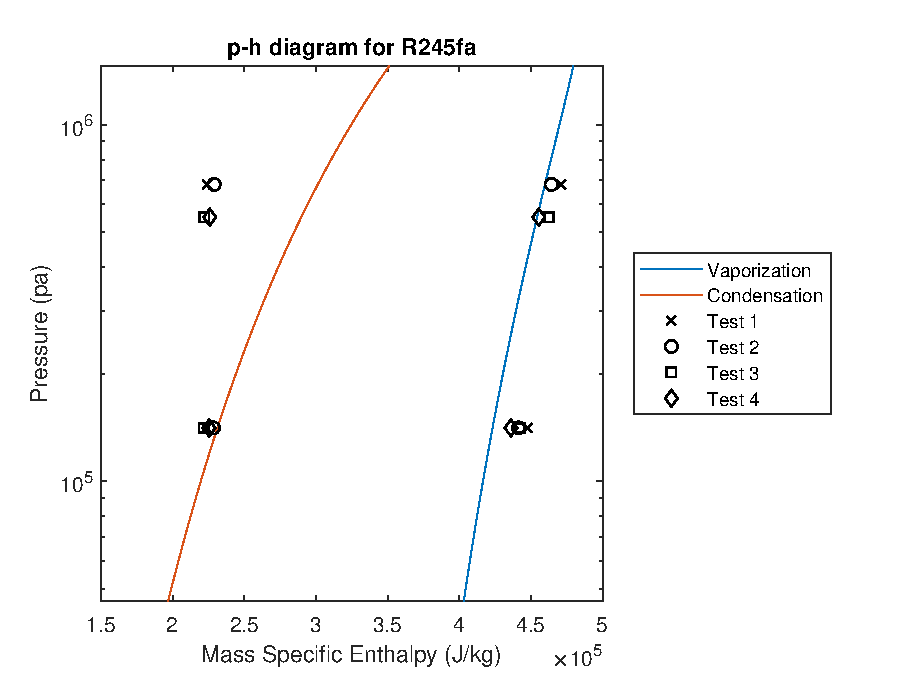
\includegraphics[width=\textwidth]{figures/VerificationPH02}
	%\includegraphics{figures/VerificationPH01}
	\caption{Pressure-Enthalpy plot of R245-fa for ORC verification with an over sized evaporator area. Input tempetures and flow rates remain the same. 
	For tests 1 \& 2 $T_{source}$ is about \SI{364}{\kelvin} (\SI{195}{\degreeFahrenheit})
	while for 3 \& 4 $T_{source}$ is \SI{353}{\kelvin} (\SI{175}{\degreeFahrenheit}). 
	In all cases $T_{sink}$ is about \SI{283}{\kelvin} (\SI{50}{\degreeFahrenheit}). 
	The hot water flow rate for tests 1 \& 3 are \SI{18.9}{\liter\per\second} (\SI{300}{\gpm})
	and	\SI{7.6}{\liter\per\second} (\SI{120}{\gpm}) for test 2 \& 4. 
	The cold water flow rate for tests 1 \& 3 are \SI{12.6}{\liter\per\second} (\SI{200}{\gpm})
	and \SI{7.6}{\liter\per\second} (\SI{120}{\gpm}) for test 2 \& 4.}
	\label{fig:verifcation_ph02}
\end{figure}
shows the lower mass flow rate of the working fluid allows it to fully vaporize due to the larger transfer area of the evaporator. 

Under four different combinations of source and sink flow rates and temperatures, the gross output power of the model matched the measured values. However, given the assumed heat transfer area of the evaporator and condenser, the power consumed by the pump was calculated to be much greater than what was measured. Increasing the area of the evaporator such that it roughly matched the condenser greatly reduced the calculated power needed by the pump. However, this is not typical for ORCs. Generally condensers are sized larger than evaporators so the system can also feasibly use air to cool the working fluid. 
\clearpage

\section{Case Study Scenarios}
With the model validated the greenfield and brownfield scenarios can be simulated and analyzed. For the former, no electrical grid is currently present, while for the latter there is existing electrical infrastructure. However, in the brownfield case the grid is not perfectly reliable. In the event of a grid outage, the microgrid should be capable of disconnecting and acting on its own. In both scenarios, the same generator impedances are used as in the validation simulations. 

\subsection{Greenfield Scenario --- Alaska}
This system is located approximately two hours north of Nome, Alaska on the western coast of the state as seen \autoref{fig:AKheatmap}, a geothermal heat map of Alaska \cite{Batir2013}. The hot water resource is drawn from the Pilgrim Hot Springs. The hot water is assumed to be drawn at a temperature of \SI{364.5}{\kelvin} (\SI{91.3}{\degreeCelsius}) and a flow rate of \SI{15.2}{\liter\per\second}. The hot water resource is fairly stable throughout the year. The low temperature water ranges from \SIrange{276.6}{281.6}{\kelvin} (\SIrange{3.5}{8.5}{\degreeCelsius}) at a flow rate of \SI{15.6}{\liter\per\second} to provide a heat sink \cite{Haselwimmer2013, AlaskaCenterforEnergyandPower2014}. Though the low temperature sink resource does vary in temperature with the seasons, the nearby geothermal activity keeps it liquid all year round.
%It is assumed the water is drawn in at atmospheric pressure.
\begin{figure}[p]
	\centering
	
	\includegraphics[width=\textwidth]{figures/AKHeatMapSMU_HFMAK2013} 

	\caption[A heat map of Alaska indicating geothermal hot spots within the state. The Pilgrim Hot Springs circled in blue. Credit: Batir et al..]{A heat map of Alaska indicating geothermal hot spots within the state. The Pilgrim Hot Springs circled in blue. Credit: Batir et al. \cite{Batir2013}.
	}
	\label{fig:AKheatmap}


\end{figure}

The assumed working fluid is R245-fa, a typical refrigerant used by a large proportion of ORC manufacturers.
% such as Electratherm, Clean Energy Technologies Inc., etc. 
The operating high and low pressure set points of the working fluid are \SIrange{570}{600}{\kilo\pascal} and \SIrange{130}{140}{\kilo\pascal}, respectively. The evaporator has a heat transfer area of \SI{37.8}{\meter\squared}, and an effective heat transfer coefficient of \SI{1500}{\watt\per\kelvin\per\meter\squared}. The condenser has an area of \SI{102.5}{\meter\squared}, but an effective heat transfer coefficient of \SI{1400}{\watt\per\kelvin\per\meter\squared}.

Four tests were conducted under different input conditions. Tests one and two use the warmer summer heat sink temperature, while tests three and four use the colder winter heat sink temperatures. Furthermore, tests one and three use the maximum power setpoint while also ensuring the working fluid fully evaporates in the evaporator, whereas in tests two and four the maxiumum power setpoint with a stable simulation is used. \autoref{fig:gfPower} compares the mechanical power, $P_{mech}$, the generator power, $P_{gen}$, inverter output power, $P_{out}$, and the electrical power consumed by the pump, $P_{pump}$, for the different tests. The working fluid mass flow rates, $\dot{m}$, are seen in \autoref{fig:gfFlow}. Finally, the heat flow rates of the evaporator and condenser, $\dot{Q}_{evap}$ and $\dot{Q}_{cond}$, are seen in \autoref{fig:gfHeat}.
\begin{figure}[p]
	\centering

	\includegraphics[width=\textwidth]{figures/gfPower}

	\caption{Comparison of mechanical power, generator power, inverter output power, and pump power consumption for the greenfield case of the ORC prime power system model. All tests assume a source temperature of \SI{364.5}{\kelvin} (\SI{91}{\degreeCelsius}), and source and sink flow rates of \SI{940}{\liter\per\minute}. Tests 1 and 2 use a heat sink temperature of \SI{281.6}{\kelvin} (\SI{8.5}{\degreeCelsius}), while tests 3 and 4 use \SI{276.6}{\kelvin} (\SI{3.5}{\degreeCelsius}). The power setpoints of the four tests are \SIlist{27.5;40.0;30.8;42.0}{\kilo\watt}. Tests 1 and 3 use the maximum power setpoint while also ensuring the working fluid fully evaporates in the evaporator. Tests 2 and 4 use the maximum power setpoint while maintaining a stable simulation. }
	%Psetpoint[2.75e4;4.0e4;3.08e4;4.2e4;]
	\label{fig:gfPower}
\end{figure}
\input{figures/gfFlow}
\input{figures/gfHeat}

Depending on the operator's tolerance of the state of the working fluid, the available gross output of the ORC prime power system can vary significantly. The gross output power of the inverter, $P_{out}$, the system can achieve while ensuring the working fluid fully vaporizes is \SIrange{28.3}{31.6}{\kilo\watt} throughout the year. In these cases the pump only needs to move about \SI{1.6}{\kilogram\per\second} consuming \SI{0.80}{\kilo\watt} of power. This yields a net output of \SIrange{27.5}{30.8}{\kilo\watt} before accounting for the power required for hot and cold water pumps. Heat is absorbed from hot water at a rate, $\dot{Q}_{evap}$, of \SIrange{361}{406}{\kilo\watt\textsubscript{th}} indicating a net efficiency 
\begin{equation}
\eta = \frac{P_{out}-P_{pump}}{\dot{Q}_{evap}}
\end{equation}
of $\eta = 7.6\%$.

More heat can be moved by increasing the working fluid flow rate yielding a greater gross power output. For flow rates of around \SI{8.4}{\kilogram\per\second}, the gross power output of the system is \SIrange{44.6}{46.2}{\kilo\watt}, with the greater end of the range occurring during the winter. Under these conditions the pump consumes about \SI{4.5}{\kilo\watt} cycling the working fluid, netting a power output of \SIrange{40.1}{41.7}{\kilo\watt}. More power is being generated because heat is being transferred at a greater rate from the source, \SIrange{751}{792}{\kilo\watt\textsubscript{th}}, but the efficiency is lower at about 5.3\%.

The drop in efficiency from 7.6\% to 5.3\% as the working fluid flow rate increases can be understood by the plots in \autoref{fig:gf_themoplots}. These plots show pressure versus temperature, pressure versus mass specific enthalpy, and temperature versus mass specific entropy using summer and winter relative ambient temperature conditions at the site. The curves in the plots represent the dividing lines between pure liquid on the left side of each plot, pure gaseous on the right, and the region where the fluid overcomes the latent heat necessary to change states in-between the curves. The points, with data markers in each of the three plots, represent the state of the working fluid between each block for the four different tests: low working fluid flow rate during summer, high flow rate during summer, low flow rate in winter, and high flow rate in winter. 
\begin{figure}[p]
	\centering

	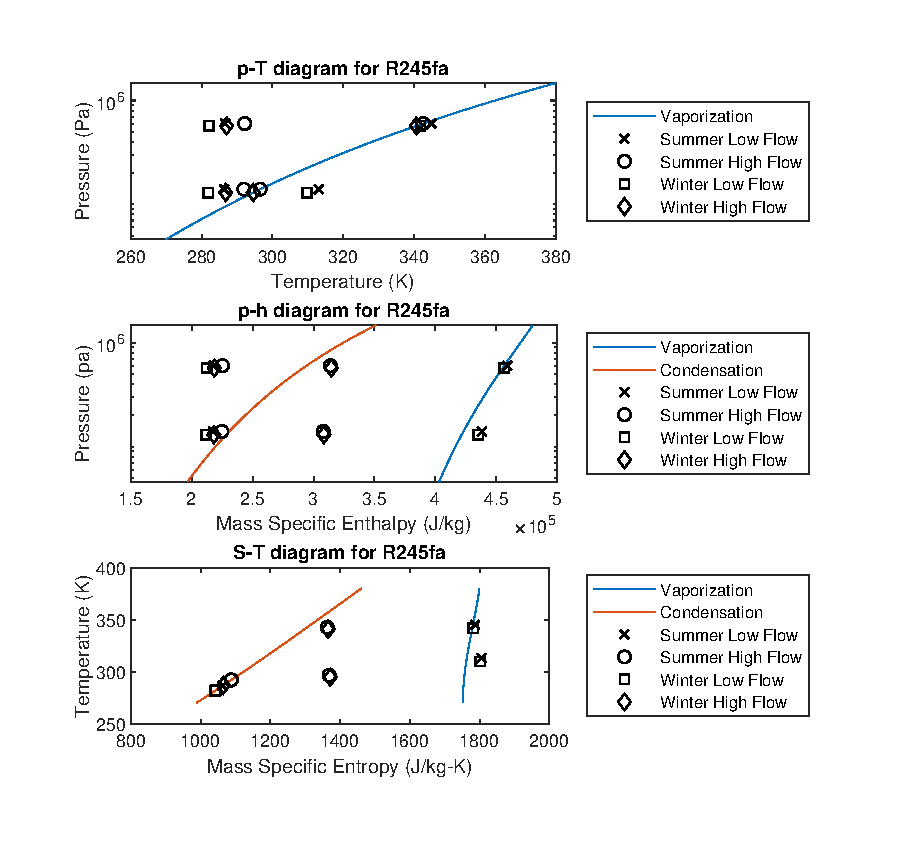
\includegraphics[width=\textwidth]{figures/GreenfieldThermoPlots}
	%\includegraphics{figures/VerificationPH01}
	\caption{Thermodynamic plots from the greenfield ORC prime power system which includes pressure against temperature (top), pressure against mass specific enthalpy (middle), and temperature against mass specific entropy (bottom). All points assume a source temperatures of \SI{364.5}{\kelvin} (\SI{91}{\degreeCelsius}), as well as source and sink flow rates of \SI{940}{\liter\per\minute}. Sink temperatures are assumed to be \SI{276.6}{\kelvin} (\SI{3.5}{\degreeCelsius}) in Winter and \SI{281.6}{\kelvin} (\SI{8.5}{\degreeCelsius}) in Summer. High flow rate points have a working fluid mass flow rate of approximately \SI{8.4}{\kilogram\per\second}}
\label{fig:gf_themoplots}
\end{figure}

The first panel (top) shows pressure (\si{\pascal}) versus temperature (\si{\kelvin}). A benefit of this plot is that it is easy to identify increases and decreases in both temperature and pressure as the working fluid moves through the cycle. However, this comes at a cost of resolution in the liquid-vapor region. In this plot the vaporization and condensation curve overlap without representing the latent heat needed to change from one phase to the other. In this particular plot there are points in this area that are not discernible despite being at different energy levels. 

The second panel (middle) helps resolve this problem by plotting mass specific enthalpy (\si[per-mode=symbol-or-fraction]{\joule\per\kilogram}) on the x-axis instead of temperature. It can be seen that the low flow rate tests allow the fluid to fully become a gas and cross the vaporization curve. Since each \si{\kilogram} of fluid contains more energy, the turbine is able to operate more efficiently, even though more total energy is being extracted at higher flow rates.

The third panel (bottom) shows temperature (\si{\kelvin}) as a function of mass specifc entropy (\si[per-mode=symbol-or-fraction]{\joule\per\kilogram\per\kelvin}). This shows the non-ideal isentropic transition of the pump and turbine. This is difficult to see for the pump because the points before and after the pump lie nearly on top of one another. Both the temperature and entropy changed very little in the process. In the turbine, however, it is clearer. Ideally the points would drop straight down on this plot, but instead there is a slight increase in entropy due to the isentropic inefficiency as expected from the 2\textsuperscript{nd} law of thermodynamics. 

The \SI{30.8}{\kilo\watt} power output could be used to operate a greenhouse nearby during the winter. Assuming about \SI{1}{\kilo\watt} of power to supply the circulation fans and watering system, as well as LED lighting of 
%\SI{3.3}{\kilo\watt\per\meter\squared} \cite{Singh2015}
\SI{650}{\watt\per\meter\squared} \cite{Tamulaitis2005} for growing plants such as lettuce and radish, then a roughly \SI{45}{\meter\squared} greenhouse could be powered entirely off the ORC system. During the summer months fewer lights, if any, are needed to grow the plants due to the longer Alaska days, therefore, the lower available power would not be a problem.
%\clearpage

\subsection{Brownfield Scenario --- Iceland}
Bergsta$\eth$ir, Iceland is located inland east of Reykjavík, as seen by the circled region on the map in \autoref{fig:Icelandheatmap}, which depicts high and low temperature geothermal resources on the island \cite{Loftsdottir2006}. The hot water resource is drawn at a flow rate of about \SI{6}{\liter\per\second} from below the surface to a holding tank before being distributed to the homes for heating. While sitting in this tank, the water is approximately \SI{368}{\kelvin} (\SI{95}{\degreeCelsius}). Nearby there is a \SI{278}{\kelvin} (\SI{5}{\degreeCelsius}) stream which can be drawn from in order to provide a low temperature sink fluid.
\begin{figure}[h]
	\centering
	
	\includegraphics[width=\textwidth]{figures/IcelandGeothermalMap} 

	\caption[A heat map of Iceland indicating high and low temperature geothermal hot spots within the country. Bergsta$\eth$ir is located in the region circled in black. Credit: Loftsdottir et al..]{A heat map of Iceland indicating high and low temperature geothermal hot spots within the country. Bergsta$\eth$ir is located in the region circled in black. Credit: Loftsdottir et al. \cite{Loftsdottir2006}.}
	\label{fig:Icelandheatmap}
\end{figure}

The working fluid is also assumed to be R245-fa. The operating high and low pressure set points of the working fluid are \SI{600}{\kilo\pascal} and \SI{140}{\kilo\pascal}, respectively. The evaporator has a heat transfer area of \SI{37.83}{\meter\squared}, and an effective heat transfer coefficient of \SI{1500}{\watt\per\kelvin\per\meter\squared}. As before, it is usual in commercial ORC systems for the condenser to have a greater area to allow for the option of air cooling. In this case the condenser has an area of \SI{37.83}{\meter\squared} and an effective heat transfer coefficient of \SI{1400}{\watt\per\kelvin\per\meter\squared}. The pump and its driving motor are assumed to have efficiencies of 70\% and 90\%, respectively. The turbine is assumed to have a mechanical efficiency of 78\% for the operating conditions.
%, while the input parameters of the generator can be seen in Fig X. 
The inverter used to convert the unregulated AC output of the self-excited induction generator to a regulated voltage output at 60 Hz is assumed to have an efficiency of 93\%.

Under these conditions, the model predicts an ORC prime power system to produce \SI{31.7}{\kilo\watt} of mechanical power, \SI{30.8}{\kilo\watt} of electrical power from the induction generator, a gross electrical power output from the inverter of \SI{28.6}{\kilo\watt}, and a working fluid pump power consumption of \SI{0.8}{\kilo\watt} as shown in \autoref{fig:bfPower}. After accounting for the power consumed to circulate the working fluid, the resultant power available for other devices on the microgrid is \SI{27.8}{\kilo\watt}. Unfortunately, this is insufficient for the desired application of this system;  running two 15 kW motors used to distribute the hot water for home heating. Additionally, this does not even take into account the pump needed to collect the low-temperature stream water for the low temperature sink.
\begin{figure}[h]
	\centering

	\includegraphics[width=\textwidth]{figures/bfPower}

	\caption{Comparison of mechanical power, generator power, inverter output power, and pump power consumption for the brownfield case of the ORC prime power system model. The test assumes a source temperature of \SI{368}{\kelvin} (\SI{95}{\degreeCelsius}) and a sink temperature of \SI{278}{\kelvin} (\SI{5}{\degreeCelsius}). The source is assumed to flow at a rate of \SI{6}{\liter\per\minute} while the sink flows at \SI{7}{\liter\per\minute}. }
	%Psetpoint[2.75e4;4.0e4;3.08e4;4.2e4;]
	\label{fig:bfPower}
\end{figure}

\autoref{fig:bf_themoplots} shows similar thermodynamic plots as for the greenfield scenario. The top right point of each plot represents the state of the working fluid as it is leaving the evaporator before entering the expander. It can be seen that this point lies on the vaporization curve. This means if the working fluid mass flow rate were to increase in order to get more power out, then the fluid would not fully vaporize and the expander efficiency assumption would no longer be valid.
If the amount of heat transferred could be increased, then it is possible the working fluid flow rate could increase as well while maintaining full vaporization. This can be achieved by increasing the heat transfer area of the evaporator. Additionally, different working fluids have different the latent heats, heat capacities, and evaporation temperatures, all of which affect the heat transfer rate.
\begin{figure}%[h]
	\centering
	\caption{Thermodynamic plots of the simulated Brownfield ORC plotting pressure against temperature, pressure against enthalpy, and temperature against entropy. Source temperature and flow rate are assumed to be \SI{95}{\degreeCelsius} and \SI{6}{\liter\per\second}. Sink temperature and flow rate are assumed to be \SI{5}{\degreeCelsius} and \SI{7}{\liter\per\second}.}
	\label{fig:bf_themoplots}
	
	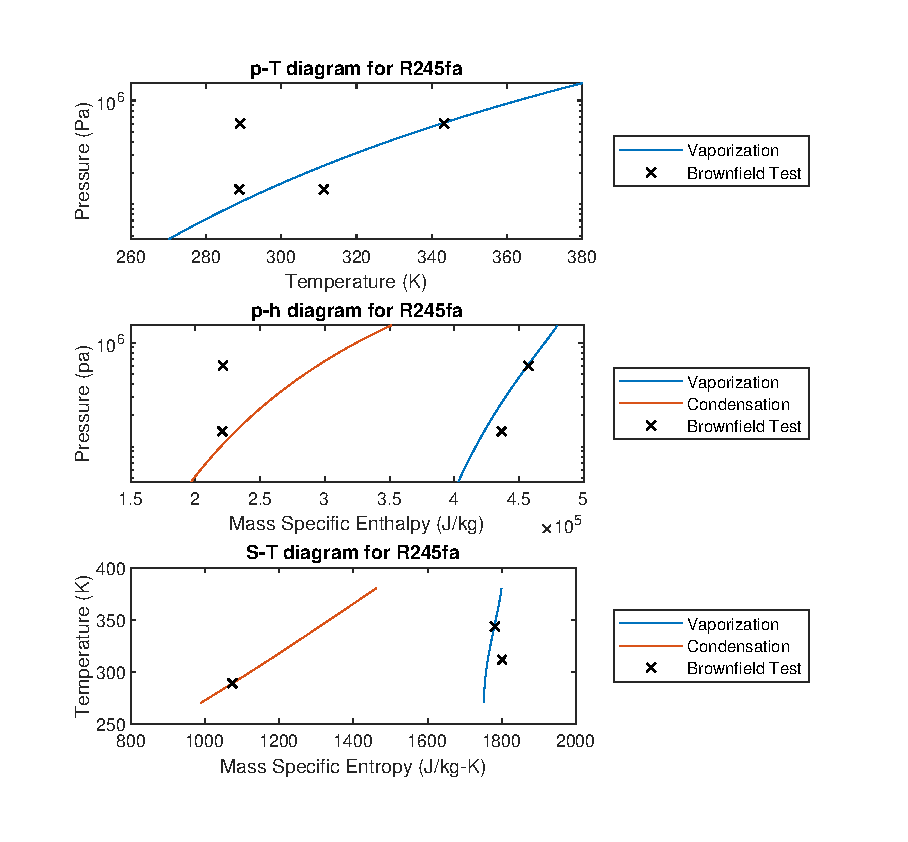
\includegraphics[width=\textwidth]{figures/BrownfieldThermoPlots}
	%\includegraphics{figures/VerificationPH01}
\end{figure}

\cleardoublepage
\chapter{Conclusion}
\label{ch:conclusion}

The goal of this thesis was to explore a viable and affordable method of incorporating renewable energy into electrical systems. Low temperature geothermal sites were looked at specifically because such sites can be found within Alaska and similar environments which are not currently fully utilized. To achieve the goal, a model was developed to simulate the thermodynamic and electrical processes. Next, two different systems were examined; a greenfield site with minimal existing infrastructure, and a brownfield site that is already electrified. 

\section{Verification}
In order to verify the model approximates reality, a Electratherm Green Machine was simulated under testing conditions. These values were compared to the results of a Green Machine test at the University of Alaska Fairbanks. There were some difficulties in re-creating exact conditions because some values were not precisely recorded. For example operating ranges for the high and low pressures of the working fluid were stated, but specific measurements were not included.
% area/U discrpencies

Under four different combinations of source and sink flow rates and temperatures, the gross output power of the model matched the measured values. However, given the assumed heat transfer area of the evaporator and condenser, the power consumed by the pump was calculated to be much greater than what was measured. Increasing the area of the evaporator such that it roughly matched the condenser greatly reduced the calculated power needed by the pump. However this is not typical for ORCs. Generally condensers are sized larger than evaporators so the system can also feasibly use air to cool the working fluid. 

\section{Greenfield}
It was shown that output of an ORC could produce a net output of around \SIrange{27.5}{30.8}{\kilo\watt} over the course of the year. This is due to a steady temperature hot water resource and a cold water sink that varies over seasons but remains liquid. According to the model, more power could be produced by increasing the flow rate. However this assumes the isentropic efficiency of the turbine expander is equal in the two cases, which is unlikely. The additional mass means the fluid does not fully vaporize, which is not typical for ORC systems because the efficiency is not constant under all conditions. Furthermore, the higher flow rate means a larger pump must be sized for the system, increasing the total cost

\section{Brownfield}
The expected net power produced by an ORC for a microgrid system is \SI{27.8}{\kilo\watt}, just under the desired \SI{30}{\kilo\watt} needed to drive the district heating pumps. However, there was sufficient power produced, but due to inefficiencies and parasitic loads there was not enough power remaining for everything. 

The gross electrical power produced by the generator before inverter losses is just shy of \SI{30.8}{\kilo\watt}. This indicates there may be enough power from the local resource to operate the district heating system while the electrical grid is active and capable of regulating the frequency and voltage of the induction generator. However the whole system would still go down during a power outage and the diesel generators would still need to be used to give the community heat.

One possible solution is to increase the size of the evaporator area. This could allow the more heat to flow from the water to the working fluid, meaning the more fluid could be moved while still fully vaporizing. Unfortunately, the cost of the system would go up as well due to larger heat exchanger.

%check the mech power produced
Another option could be to bypass electrical conversion entirely, eliminating several inefficiencies along the way. The simulated ORC produced about \SI{31.7}{\kilo\watt} of mechanical power, and the \SI{30}{\kilo\watt} district heating pumps actually need slightly less mechanical power to operate. A system could be developed to connect the ORC expander directly to a mechanical pump to drive the district heating loop. Other inefficiencies would likely be introduced and controlling the flow would be challenging, but it might be worth further examination.

\section{Future Work}
\subsection{Thermal Model}
As described previously, more heat was transferred through the heat exchangers in the model than what was measured in trials. A possible explanation is that the model is perfectly efficient at transferring the heat and none is lost to the ambient environment. The overall accuracy of the model could be improved by accounting for this additional route of heat flow.

Another implementation that could improve system performance is an optional pre-heater that several commercial systems already use. This heat exchanger is inserted in the loop between the pump and evaporator on the high pressure side effectively increasing the area of the evaporator. Sometimes the pre-heater uses a different heat source from the primary source. Even the heat of the working fluid coming off of the expander before flowing through the condenser could be used. This allows the system to recycle some of the heat that was not converted into mechanical energy letting it operate at a slightly higher efficiency at the cost of an additional component.

\subsection{Electrical Model}
The microgrids simulated as a part of this project only included squirrel cage induction generators because they are relatively inexpensive to build and maintain and are therefore commonly used in commercial ORC systems. They are not, however, ubiquitous. It would be beneficial for future works to include models of additional generator types such as DC or permanent magnet synchronous machines. This could allow the user to compare systems made by different manufacturers and which use alternative technologies.
%various inverter models
%add storage

\subsection{Transient Model}
This model was designed to examine steady-state results. It looks at the energy balance of each component to simulate how they interact over long term. This means it is unable to accurately capture transient dynamics after a change in load, temperature, or flow rate. Each of those fluctuations may operate at different time scales and effect the system differently. It is important to know the system is capable of providing primary power while maintaining grid frequency and voltage under those different perturbations.


\bibliographystyle{ieeetr}
\bibliography{NG_bib}

\end{document}
